\documentclass[11pt,a4paper,oldfontcommands,oneside]{memoir}
\usepackage[utf8]{inputenc}
\usepackage{microtype}
\usepackage[dvips]{graphicx}
\usepackage{xcolor}
\usepackage{times}
\usepackage{graphicx}
\usepackage[spanish]{babel}
\usepackage[
breaklinks=true,colorlinks=true,
%linkcolor=blue,urlcolor=blue,citecolor=blue,% PDF VIEW
linkcolor=black,urlcolor=black,citecolor=black,% PRINT
bookmarks=true,bookmarksopenlevel=2]{hyperref}

\usepackage{geometry}
% PDF VIEW
% \geometry{total={210mm,297mm},
% left=25mm,right=25mm,%
% bindingoffset=0mm, top=25mm,bottom=25mm}
% PRINT
\geometry{total={210mm,297mm},
left=20mm,right=20mm,
bindingoffset=10mm, top=25mm,bottom=25mm}

\OnehalfSpacing
%\linespread{1.3}

%%% CHAPTER'S STYLE
\chapterstyle{bianchi}
%\chapterstyle{ger}
%\chapterstyle{madsen}
%\chapterstyle{ell}
%%% STYLE OF SECTIONS, SUBSECTIONS, AND SUBSUBSECTIONS
\setsecheadstyle{\Large\bfseries\sffamily\raggedright}
\setsubsecheadstyle{\large\bfseries\sffamily\raggedright}
\setsubsubsecheadstyle{\bfseries\sffamily\raggedright}


%%% STYLE OF PAGES NUMBERING
%\pagestyle{companion}\nouppercaseheads 
%\pagestyle{headings}
%\pagestyle{Ruled}
\pagestyle{plain}
\makepagestyle{plain}
\makeevenfoot{plain}{\thepage}{}{}
\makeoddfoot{plain}{}{}{\thepage}
\makeevenhead{plain}{}{}{}
\makeoddhead{plain}{}{}{}


\maxsecnumdepth{subsection} % chapters, sections, and subsections are numbered
\maxtocdepth{subsection} % chapters, sections, and subsections are in the Table of Contents


%%%---%%%---%%%---%%%---%%%---%%%---%%%---%%%---%%%---%%%---%%%---%%%---%%%

\begin{document}

%%%---%%%---%%%---%%%---%%%---%%%---%%%---%%%---%%%---%%%---%%%---%%%---%%%
%   TITLEPAGE
%
%   due to variety of titlepage schemes it is probably better to make titlepage manually
%
%%%---%%%---%%%---%%%---%%%---%%%---%%%---%%%---%%%---%%%---%%%---%%%---%%%
\thispagestyle{empty}

{%%%
\sffamily
\centering
\Large

~\vspace{\fill}

\includegraphics[scale=1]{logo1.png} \\
{\huge 
\vspace{4cm}
Describir los métodos geométrico, algebraico y desacoplo cinemático
}
\vspace{2.5cm}

{\LARGE
Eduardo Robles Vázquez
}

\vspace{2.5cm}

Universidad Politécnica de la Zona Metropolitana de Guadalajara

\vspace{3.5cm}

Profesor: Carlos Enrique Morán Garabito

\vspace{\fill}

22 de Octubre de 2019

%%%
}%%%

\vspace{.5cm}
\hfill\break




\tableofcontents*

\clearpage

%%%---%%%---%%%---%%%---%%%---%%%---%%%---%%%---%%%---%%%---%%%---%%%---%%%
%%%---%%%---%%%---%%%---%%%---%%%---%%%---%%%---%%%---%%%---%%%---%%%---%%%
\chapter{Método Geométrico}
Los métodos geométricos permiten tener normalmente los valores de las primeras variables articulares, que son las que consiguen posicionar el robot. Para ello utilizan relaciones trigonometrías y geométricas sobre los elementos del robot. Se suele recurrir a la resolución de triángulos formados por los elementos y articulaciones del robot. 
\\

Es adecuado para robots de pocos grados de libertad o para el caso de que se consideren solo los primeros grados de libertad para posicionar el extremo. El procedimiento se basa en encontrar un número suficiente de relaciones geométricas en las que intervendrán las coordenadas del extremo del robot, sus coordenadas articulares y las dimensiones físicas de sus elementos:\\
 
---Robot con 3 grados de libertad.

---Coordenas $P_x$, $P_y$, $P_z$ 

---Robot con estructura planar.\\
 
La orientación del último eslabón es la suma de las variables articulares.

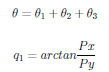
\includegraphics[scale=1.5]{1} 

Considerando ahora únicamente r y utilizando el teorema del coseno, se tendrá:

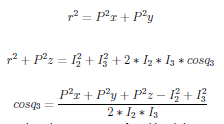
\includegraphics[scale=1.5]{2}\\


Esta expresión permite obtener q1 en función del vector de posición del extremo P. No obstante, por motivos de ventajas computacionales, es más conveniente utilizar la expresión de arco tangente en lugar del arco seno. Puesto que: 

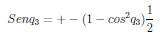
\includegraphics[scale=1.5]{3}

Se tendrá que: 

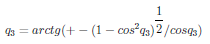
\includegraphics[scale=1.5]{4}\\
  
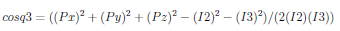
\includegraphics[scale=1.5]{5} 

El cálculo de $q_2$ se hace a partir de la diferencia entre $ß$ y $a$:\\

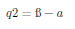
\includegraphics[scale=1.5]{6} 

Siendo:

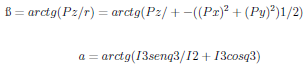
\includegraphics[scale=1.5]{7} 


Luego:

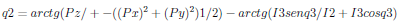
\includegraphics[scale=1.5]{8} 

De nuevo los dos posibles valores según la elección del signo dan lugar a dos valores diferentes de q2 correspondientes a las configuraciones codo arriba y abajo.

\chapter{Método Algebraico}
Resolución a partir de las matrices de transformación homogénea\\ 
---Se resuelve la cinemática directa y se obtienen las matrices A.\\
---Para evitar la aparición de ecuaciones trascendentes,se va  premultiplicando por las matrices inversas.\\
---Se intenta obtener de esta forma una ecuación que aísle en uno  de los lados una de las variables articulares.\\
---La elección de los elementos ha de realizarse con sumo cuidado.\\
---Por su complejidad a menudo este método se deshecha.\\


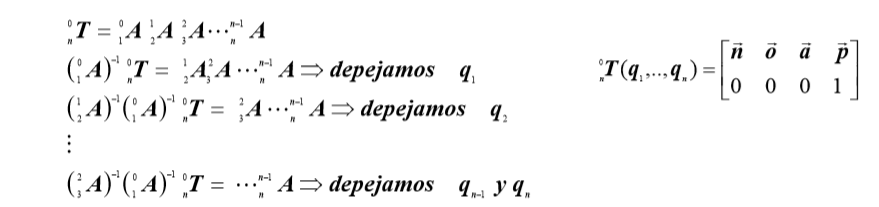
\includegraphics[scale=.5]{ec3.png}

Se trata de igualar elementos de ambos lados de cada ecuación, tomando los casos en los que solo aparezca una variable de articulación, empleando identidades trigonométricas y buscando divisiones en función de arco tangentes. \\

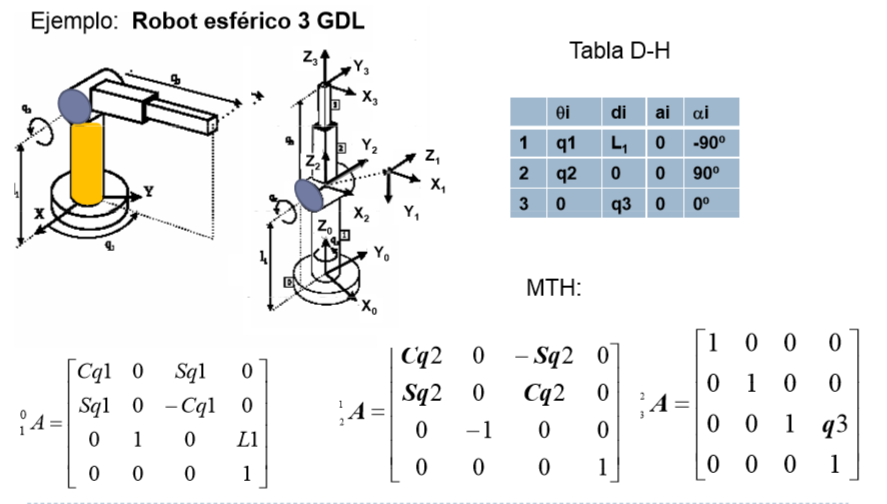
\includegraphics[scale=.5]{robot.png} \\

\chapter{Método Desacoplo Cinemático}
\begin{center}
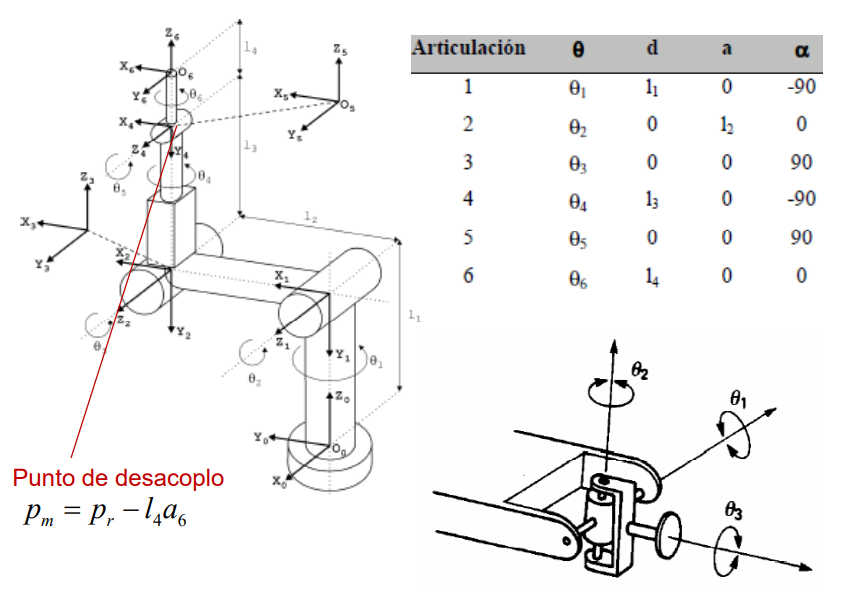
\includegraphics[scale=.5]{robot22}
\end{center}
 

Aplicable en robots donde los últimos 3 grados de libertad cortan en un mismo punto, la muñeca.\\

El método de desacoplamiento cinemático permite, para determinados tipos de robots, resolver los primeros grados de libertad, dedicados al posicionamiento, de una manera independiente a la resolución de los últimos grados de libertad, dedicados a la orientación. Si bien la variación de estos tres últimos grados de libertad origina un cambio en la posición final del extremo real del robot, su verdadero objetivo es poder orientar la herramienta del robot libremente en el espacio. \\

El método de desacoplo cinemático saca partido de este hecho, separando ambos problemas: Posición y orientación.  Para ello, dada una posición y orientación final deseadas, establece las coordenadas del punto de corte de los 3 últimos ejes calculándose los valores de las tres primeras variables articulares ($q_1$, $q_2$, $q_3$) que consiguen posicionar este punto. \\

A partir de los datos de orientación y de los ya calculados ($q_1$, $q_2$, $q_3$) se obtiene los valores del resto de las variables articulares. Para esta clase de manipuladores la cinemática inversa se puede resumir por el siguiente algoritmo: \\

---Paso 1: Encontrar $q_1$, $q_2$, $q_3$ de tal manera que la muñeca de centro Oc tiene coordenadas dadas por: \\

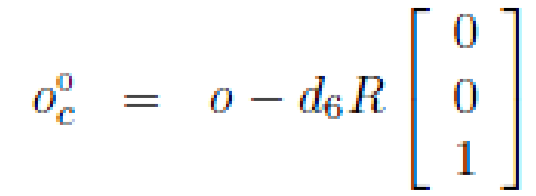
\includegraphics[scale=.35]{ec1.png} \\

---Paso 2: Usando las variables determinadas en el paso 1, evaluar $0R3$. \\

---Paso 3: Buscar un conjunto de ángulos de Euler correspondientes a la matriz de rotación.\\

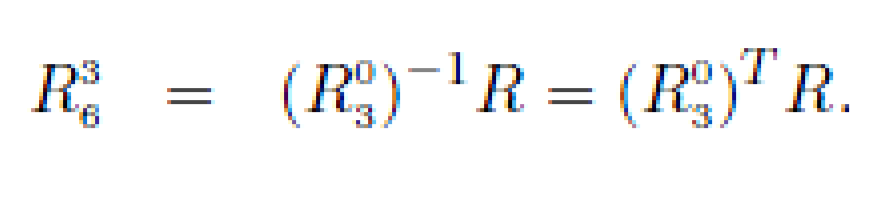
\includegraphics[scale=.25]{ec2.png} \\

\bibliographystyle{plain}
\bibliography{bibliografia}


\end{document}

